\chapter[Occupation Resolved Conductance of the Kondo Effect]{Occupation Resolved Conductance of the Kondo Effect}\label{cha:mixed_valence_conductance}
% Probably should be called: Occupation resolved conductance of the Kondo effect

\epigraph{Before I came here I was confused about this subject. Having listened to your lecture I am still confused. But on a higher level.}{Enrico Fermi}

To my knowledge, the following work in this chapter is the first time that conductance and charge transitions have been simultaneously measured to resolve the conductance enhancement due to the Kondo effect, as a function of the occupation, in an experiment. The conductance enhancement from Kondo, is most pronounced when the quantum dot is strongly coupled ($\mathrm{\Gamma/k_BT}>>1$) to the source and drain leads. Previous measurements of the Kondo effect have focused on the conductance enhancement in the middle of Coulomb blockade valleys. However, when the coupling is strong, the measured charge transitions broaden and they become difficult to convert into occupation. The following work falls between the tightly confined window of strong coupling to see the Kondo effect and weak coupling where charge transitions are easily measured. 

\section{Introduction}
Previous measurements of the Kondo effect in quantum dots have studied the temperature dependence of conductance in the middle of the Coulomb blockade valley. In this regime, the full charge of the electron is in the dot so there is a definite net spin and the theory is well understood~\cite{kondo_unitary, costi_kondo_mv_eo_regime}. In the Kondo regime, the Kondo temperature Eq.~\ref{eq:kondo_temp}, sets a new, many-body scale and is used to universally scale the conductance Eq.~\ref{eq:kondo_conductance}. This one-parameter scaling of the conductance in the Kondo regime is used as one of the demonstrations of the Kondo effect. When the coupling between the quantum dot and source and drain reservoirs is reduced, the Kondo temperature drops below the system temperature, and the conductance enhancement is not seen in the middle of Coulomb blockade valley. Few experiments have studied this region of parameter space~\cite{goldhaber_mv}. Such studies observed the parameter $\mathrm{s}$ Eq.~\ref{eq:kondo_conductance} and found that in the Kondo regime (the full charge of the electron is in the dot), $\mathrm{s}$ was constant and equal to $0.20$. However, $\mathrm{s}$ varied rapidly as $\tilde{\epsilon}_0>-0.5$. Qualitatively, this regime is entered when the dot energy $\epsilon_0$ approaches the Fermi energy of the leads and only a fraction of the electron charge is in the dot. 


We aimed to measure the Kondo effect with a strength of coupling such that the conductance in the Coulomb blockade valley in between conductance peaks was zero. Due to the relatively small $\Gamma$, the Kondo temperature far from the Fermi energy of the leads was very small and no conductance enhancement would be measured. However, as the dot energy approaches the Fermi energy of the leads, the Kondo temperature increases. Hence, for relatively small coupling strengths, the Kondo effect shows up as a very small enhancement of conductance on the odd occupied side of conductance peaks. As the conductance enhancement in this regime is very small, only a measurement of conductance is not sufficient to investigate the Kondo effect for two reasons. Firstly, entropy shifts the occupation of the quantum dot with temperature. This effect is taken advantage of in a recently developed entropy measurement technique~\cite{hartman, child_strong, child_meas}. This shift in occupation can be ignored when the coupling is strong and conductance enhancement in the Coulomb blockade valley is large. Secondly, charge motion in the dopant layer can shift the conductance left or right, with respect to the gate voltage. The shifting from charge motion renders it impossible to retroactively shift the conductance to offset the effects of entropy. 

For these two reasons, it is necessary to simultaneously measure a second `reference' signal alongside the conductance. This reference signal can then be used to offset the above effects and allow for comparison of the conductance across multiple temperatures. We measure the charge in the quantum dot simultaneously with conductance. Assuming a linear relation between the measured change in charge and the real occupation of the quantum dot, the charge transition is converted into an occupation. The occupation is used to plot the conductance as a function of occupation. Where a shifting of the conductance maximum to a higher occupation is a signature of the Kondo effect. To verify Kondo enhancement, a comparison to Numerical Renormalisation Group (NRG) is required. 




\section{Fitting Conduction and Charge Transitions to Theory}
To investigate the small enhancement of conductance due to the Kondo effect with relatively small coupling, the conductance and charge of the quantum dot are simultaneously measured. A simultaneous measurement of the charge and conductance is trivial on the hardware side. Two different current amplifiers are connected to the device, to measure the conductance through the quantum dot and current through the charge sensor. Each current amplifier is connected to two different analog-to-digital converters (ADCs), which sample data points simultaneously. It is much trickier to tune the quantum dot into a regime where both the conductance and charge transition can be used for comparison to theory. When weakly coupled ($\mathrm{\Gamma/k_BT}<<1$), the charge transitions have a sharp drop in current and can be fit analytically Eq.~\ref{eq:cs_lineshape}. However, conductance becomes sharply peaked and the conductance amplitude drops with the strength of coupling, 

\begin{equation}\label{eq:cond_amp}
 \mathrm{G_0} = 
 \frac
 {\Gamma_\mathrm{L}\cdot\Gamma_\mathrm{R}}
 {\Gamma_\mathrm{L} + \Gamma_\mathrm{R}}
\end{equation}

Where $\mathrm{G_0}$ is the conductance maximum. Also, with reduced coupling, the conductance enhancement due to Kondo can become negligible. Additionally, the decrease in conductance amplitude means that the conductance signal can be lost within the background noise.


Alternatively, stronger coupling increases the Kondo temperature, leading to measurable enhanced conductance. However, strongly coupled charge transitions become very broadened Fig.~\ref{fig:ch1/virtual_gate_example}. Hence, when strongly coupled, large sweeps in gate voltage are required to cover the range where the quantum dot is unoccupied to fully occupied. Due to the cross-capacitive coupling between the sweep gate and the charge sensor, the change in current through the charge sensor can be pushed into a non-linear regime. A non-linear relationship between the current through the charge sensor and the addition of charge into the quantum dot makes an extraction of dot occupation from the charge transition unreliable. Hence, a virtual gate that keeps the current through the charge sensor constant is required Fig.~\ref{fig:ch1/virtual_gate_example}. The exact ratio of gates used to form the virtual gate can drastically change the underlying shape of the charge transition, this is discussed in an upcoming section. 


\subsection{Numerical Renormalisation Group (NRG)}
The dot is carefully tuned to a coupling regime where enhancement of the conductance due to Kondo is expected and charge transitions are reliably measured. As previous tests of the Kondo effect are not possible in this regime, a comparison to Numerical Renormalisation Group (NRG) calculations~\cite{nrg} is required. These calculations are provided by our theory collaborators (Yigal Meir, Yaakov Kleeorin, and Andrew Mitchell). 
Two 2d datasets corresponding to conductance and occupation are received. NRG occupation is converted to a charge transition for comparison to data. The columns are energy scaled by $\Gamma$ (energy/$\Gamma$) so that the x-axis is unit less. The rows in the 2d datasets correspond to a different value of $\mathrm{\Gamma/T}$. We confirmed with Yaakov that the lineshape does not change if both $\mathrm{T}$ and $\mathrm{\Gamma}$ increase together, that is, the lineshape really represents the ratio $\mathrm{\Gamma/T}$ not $\mathrm{\Gamma}$ or $\mathrm{T}$ individually.

To compare NRG to data, $\mathrm{\Gamma/T}$ should be reliably determined so the correct row from NRG is used. Then the correct scaling is applied to convert the NRG into the units of the measurement. Conductance and charge transitions have similar scaling parameters. Leverarm, which scales the NRG x-axis to be in units of mV, amplitude, and x offset term. The occupation NRG has extra parameters, a y offset which is the current through the charge sensor, a linear term which is the cross capacitance between the sweep gate and charge sensor, and an occupation-dependent linear term. The occupation-dependent linear term was added as we noticed a change in cross capacitance from the additional charge of an electron in the quantum dot. Many of these parameters have little cross-correlation when fitting data to NRG, meaning the global minimum of the minimiser is reliably reached. However, changes to $\mathrm{\Gamma/T}$ can be offset by a change to the leverarm, and fitting a single trace allowing both parameters ($\mathrm{\Gamma/T}$ and leverarm) to freely vary is inconsistent. 

\begin{figure}[!bht]
 \begin{center}
%% includegraphics: comment the following if not using the graphicx package
 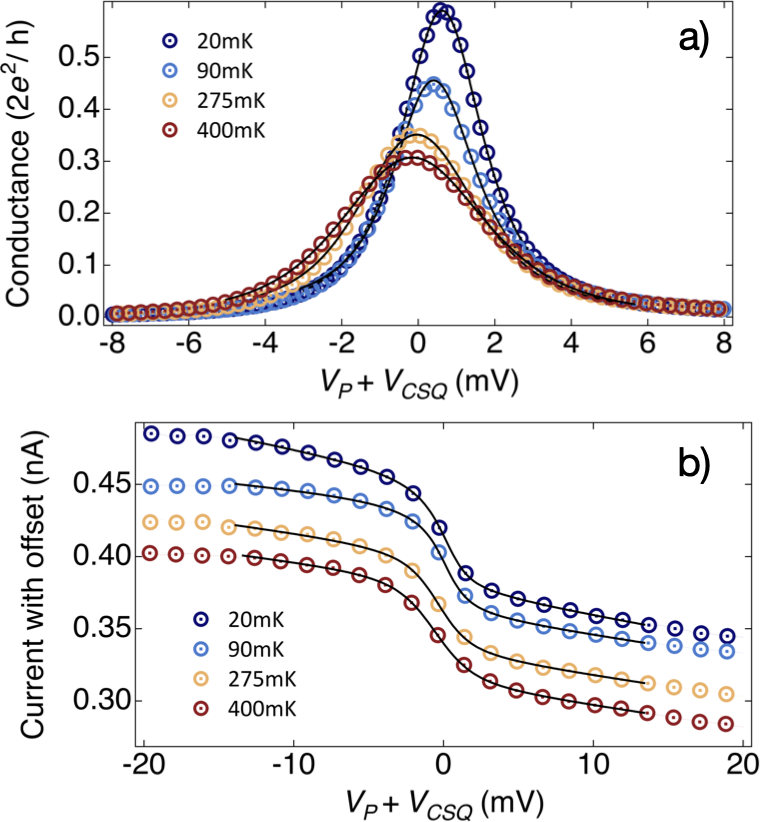
\includegraphics[width=0.8\textwidth]{figures/ch3/crop_FiguresMaster.013.png}
 \caption[Method to determine gamma and leverarm and fit to charge transitions]{\label{fig:ch3/cond_ct_gf} 
 % For some options that work with pdf\LaTeX, please see this discussion:
 % \url{http://tex.stackexchange.com/questions/11839}. 
 (\textbf{a}) Conductance data as a single electron enters a strongly coupled ($\mathrm{\Gamma/k_BT > 1}$) quantum dot, at four different temperatures. The x location of the conductance maxima has not been shifted and is the original x location of the measured data. The fits (in grey) are from a global fit to NRG, where the gamma and leverarm parameters are held fixed across all four temperatures. (\textbf{b}) Charge transitions are measured simultaneously with the conductance. Each charge transition is separately fit to NRG, where the gamma and leverarm parameters are held fixed to the values determined from the global fit to conductance.}
 \end{center}
\end{figure}

\subsection{Fitting Conductance to NRG}
In the temperature broadened regime ($\mathrm{\Gamma/T} < 1$), $\mathrm{\Gamma/T}$ and leverarm are decoupled as the broadening of the conductance or charge transition is from temperature only. To access the temperature broadened regime from the gamma broadened regime ($\mathrm{\Gamma/T} > 1$), the temperature of the fridge is increased until $\mathrm{\Gamma/T} \lesssim 1$. Data is taken at multiple temperature setpoints across this range so that $\mathrm{\Gamma/T}$ and leverarm can be reliably determined Fig.~\ref{fig:ch3/cond_ct_gf}. Conductance and charge transitions are simultaneously measured at each temperature. However, it is the conductance data that is used to determine $\mathrm{\Gamma/T}$ and leverarm, as it is, in general, cleaner. A global fit to the conductance data including each of the temperature setpoints is used in Fig.~\ref{fig:ch3/cond_ct_gf}\textbf{a}. Where $\mathrm{\Gamma}$ and leverarm are allowed to vary, but held fixed between temperatures and $\mathrm{T}$ is held fixed to the calculated electron temperature at each fridge temperature Fig.~\ref{fig:ch1/electron_temp}. The other parameters (amplitude and x offset) used to fit the NRG to conductance data are allowed to freely vary.
The fitting range is chosen to be the full width at $90\%$ the maximum conductance. This removes any bias of picking a `good' fitting range. 

\subsection{Fitting Charge Transitions to NRG}
The global fit to conductance is used to determine the parameters $\mathrm{\Gamma/T}$ and leverarm, which are then used in the fits to the charge transitions. Each charge transition is fit separately, where $\mathrm{\Gamma/T}$ and leverarm determined from the conductance global fit, are held fixed. All other parameters (amplitude, x offset, y offset, linear and occupation dependant linear) are allowed to freely vary Fig.~\ref{fig:ch3/cond_ct_gf}\textbf{b}. The fitting range of the charge transitions is maximised up to, but excluding charge jumps.


\subsection{Determining Occupation from Charge Transitions}


The charge transition cannot be used as a reference to compare with conductance, due to changing amplitude and linear terms with changes in dot settings. However, the charge transition can be converted into an occupation which allows for comparison of conductance enhancement between dot settings. The fit parameters from the NRG fit to the charge transitions are used to remove relevant terms. The current offset (y offset) and linear term are removed trivially. The occupation dependant linear term is removed by multiplying this linear term, with the correct NRG occupation row corresponding to $\mathrm{\Gamma/k_BT}$. Lastly, the charge transition is re-scaled by the amplitude. To compare the occupation data with NRG occupation. The NRG corresponding to the correct $\mathrm{\Gamma/k_BT}$ only has to be shifted by the x offset and scaled by the leverarm, as it is already in units of occupation Fig.~\ref{fig:ch3/cond_vs_occ_gf}\textbf{a}.


\subsection{Conductance versus Occupation Varying Temperature}
The data is then plotted as conductance versus occupation Fig.~\ref{fig:ch3/cond_vs_occ_gf}\textbf{b}. As the conductance and occupation data are fit to different ranges, it is important to ensure conductance and occupation data points plotted against each other correspond to the same gate voltage. Plotting conductance versus occupation solves the issue of conductance shifting with respect to the gate voltage due to entropy or charge motion. Conductance enhancement due to Kondo can be seen from a shift of the conductance maximum to occupation greater than 0.5 (N $>0.5$). This shift in the conductance maximum indicates that even as the dot energy of the quantum dot falls below the energy level of the leads, there is enhanced conductance due to the formation of a Kondo singlet. In Fig.~\ref{fig:ch3/cond_vs_occ_gf}\textbf{b}, as the temperature is lowered, the conductance maximum shifts to higher occupation. This is because the system temperature falls below the Kondo temperature and the Kondo singlet remains formed. The NRG conductance versus occupation in Fig.~\ref{fig:ch3/cond_vs_occ_gf}\textbf{b}, is the unscaled NRG provided by the theorists corresponding to $\mathrm{\Gamma/k_BT}$. There is good agreement between the data and NRG at each of the temperatures. 

\begin{figure}[!bht]
 \begin{center}
 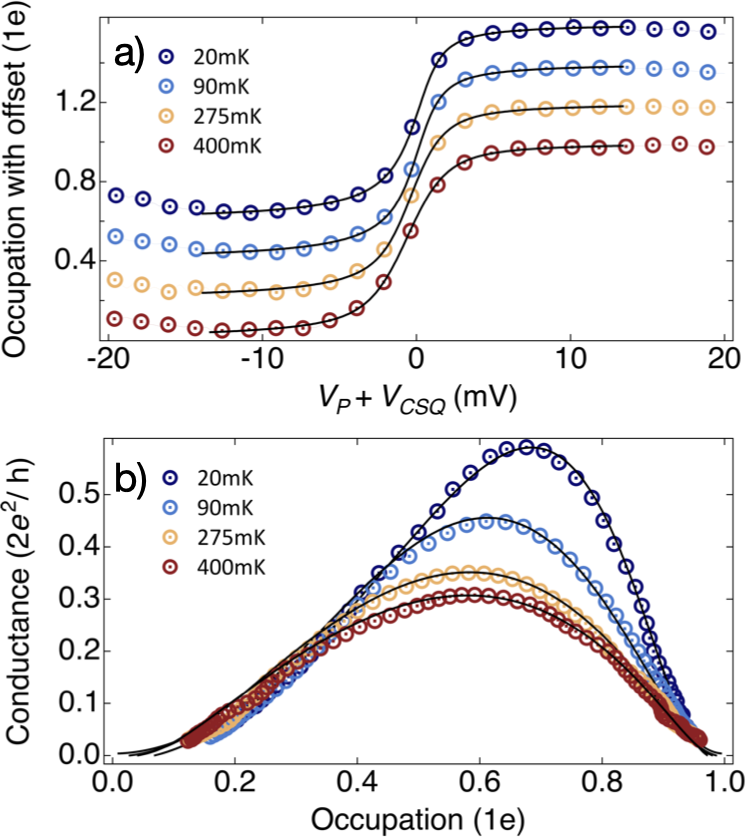
\includegraphics[width=0.8\textwidth]{figures/ch3/crop_FiguresMaster.014.png}
 \caption[Method to determine occupation and plot conductance vs. occupation]{\label{fig:ch3/cond_vs_occ_gf} 
 % For some options that work with pdf\LaTeX, please see this discussion:
 % \url{http://tex.stackexchange.com/questions/11839}. 
 (\textbf{a}) Charge transitions are converted to occupation by removing the relevant fit parameters. These are amplitude, current offset, cross capacitance of virtual gate, and occupation dependant cross capacitance. (\textbf{b}) A plot of conductance versus occupation is used to show the enhanced conductance due to Kondo. As temperature decreases, the conductance maxima occurs at greater occupation. The NRG (grey) conductance versus occupation corresponding to the determined $\mathrm{\Gamma/k_BT}$ is plotted on top of the data where good agreement is found at each temperature.}
 \end{center}
\end{figure}


\section{Conductance versus Occupation Varying Coupling Strength}


In Fig.~\ref{fig:ch3/cond_vs_occ_gf}\textbf{b}, the Kondo enhancement dependence on the temperature of the system was confirmed. Where at high temperatures $\mathrm{T>T_K}$, there is no Kondo singlet and so the conductance maximum is near $\mathrm{N} = 0.5$. But at low temperatures $\mathrm{T<T_K}$, a Kondo singlet is formed, and the conductance maximum shifts to higher occupation $\mathrm{N} > 0.5$. This displays the dependence of the Kondo temperature on the dot energy. As the dot energy gets close to the leads, the Kondo temperature rises. However, the Kondo temperature also depends on the strength of coupling between the quantum dot and leads Eq.~\ref{eq:kondo_temp}. Where strongly coupled quantum dots have larger Kondo temperatures. Hence, in strongly coupled quantum dots, the conductance maximum is expected to occur at higher occupation than in weakly coupled quantum dots. 


\begin{figure}[!bht]
 \begin{center}
%% includegraphics: comment the following if not using the graphicx package
 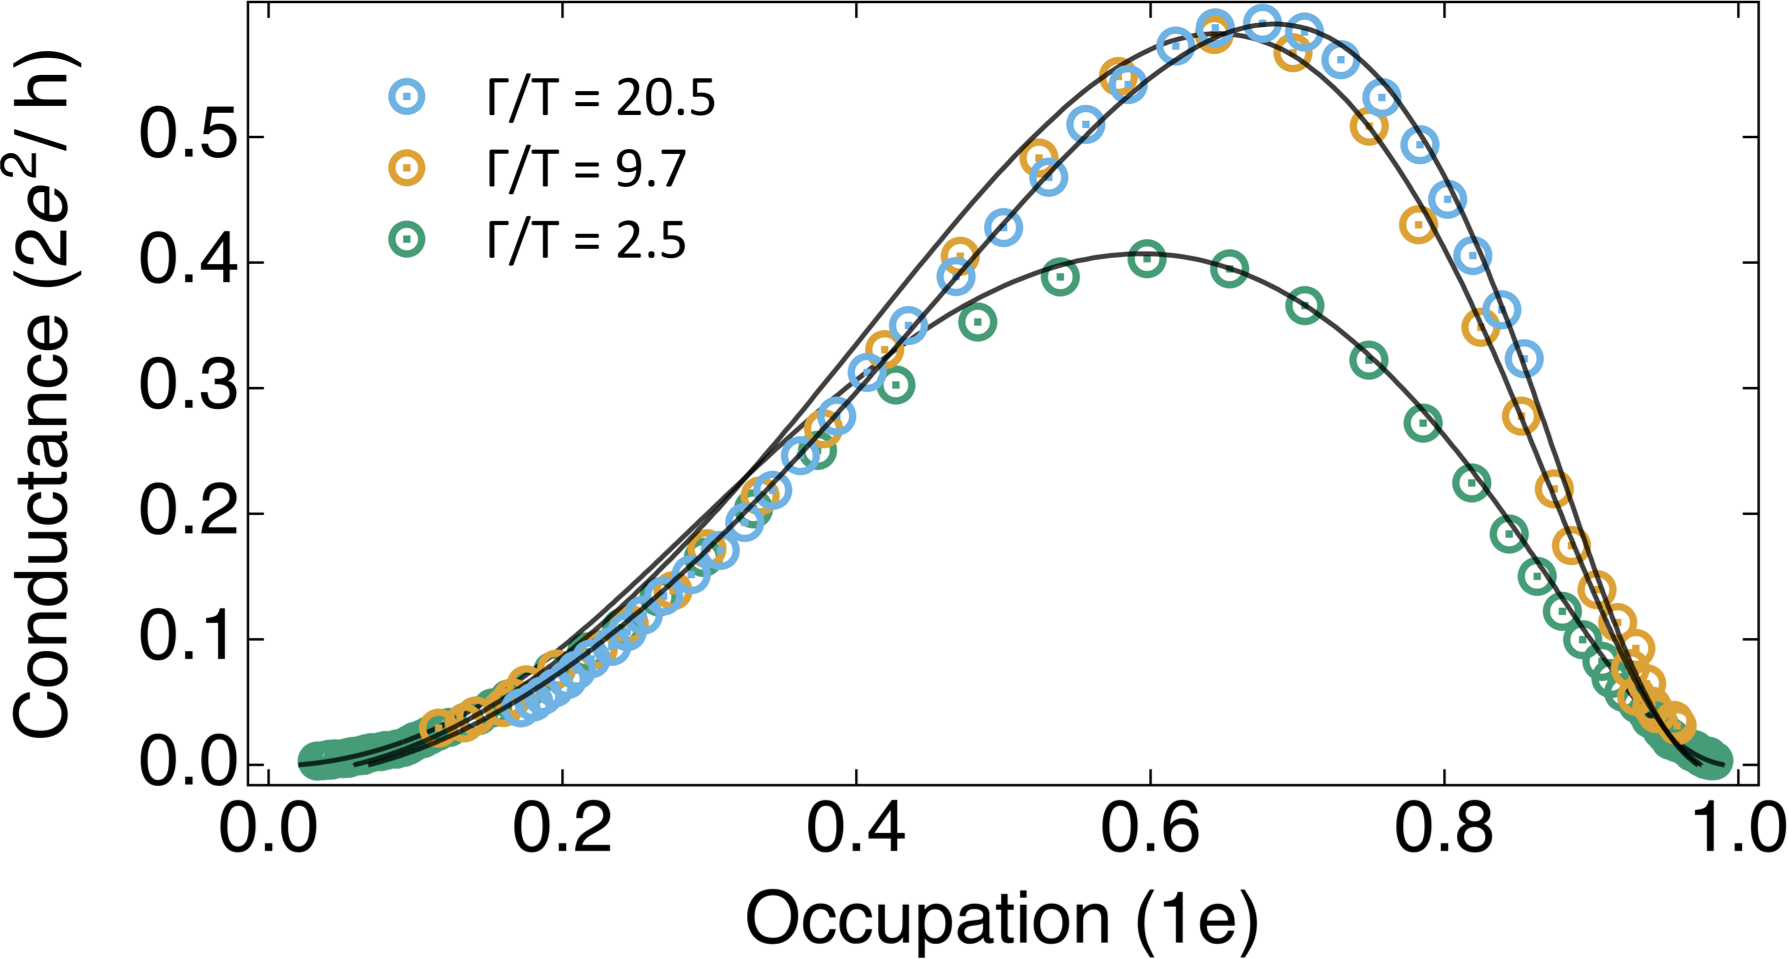
\includegraphics[width=0.8\textwidth]{figures/ch3/crop_FiguresMaster.015.png}
 \caption[Conductance vs. Occupation : Varying the coupling strength between the quantum dot and leads]{\label{fig:ch3/cond_occ_couplingstrength} 
 % For some options that work with pdf\LaTeX, please see this discussion:
 % \url{http://tex.stackexchange.com/questions/11839}. 
 Conductance versus occupation in a weak (green) and strong (blue) coupling regime. Each trace is taken at \qty{20}{mK}. The coupling strength $\mathrm{\Gamma/k_BT}$ was determined from a global fit to multiple temperatures. The NRG (grey) conductance versus occupation corresponding to the determined $\mathrm{\Gamma/k_BT}$ is plotted on top of the data where good agreement is found at each coupling strength.}
 \end{center}
\end{figure}


Fig.~\ref{fig:ch3/cond_occ_couplingstrength} shows \qty{20}{mK} traces of conductance versus occupation at three different coupling strengths. $\mathrm{\Gamma/k_BT}$ is determined using the fitting routine described above so the corresponding NRG can be plotted alongside the data. The expected behaviour, of a greater shift in the conductance maximum to higher occupation in the more strongly coupled data, is found. Good agreement with NRG is observed at each coupling.







% \afterpage{\clearpage}
% \afterpage{}
% \FloatBarrier
\section{Varying Charge Sensor Current}

This new method of plotting conductance versus occupation requires a reliable determination of $\mathrm{\Gamma/k_BT}$ and leverarm from conductance data, and clean charge transitions that can be converted into an occupation. The shape of the charge transition can vary depending on the choice of virtual gate and the charge sensor QPC setpoint. In the next section, different current setpoints of the charge sensor QPC are measured and the resulting conductance versus occupation is tested for agreement with NRG.

% \afterpage{\clearpage}
\subsection{Charge Transition Dependence on Charge Sensor Current}

Fig.~\ref{fig:ch3/cond_occ_ct_set-points} shows the underlying charge sensor QPC trace in green. Plotted on top (in yellow), are the resulting charge transitions if the charge sensor gates were set to the corresponding current through the QPC. The current (y-axis), has not been scaled differently between the charge sensor QPC trace and charge transitions. However, the sweep gate (x-axis) of the charge sensor QPC and charge transitions are not the same. The charge transition sweep gate axis has been scaled for clarity in this plot. 



The shape of the charge transition varies significantly as the current setpoint through the charge sensor QPC is changed. Normally, the QPC is set to its steepest slope, where the derivative of the QPC trace is the largest. Here, the charge sensor is most sensitive as small changes in the potential result in large changes in the current. The resulting amplitude of the charge transition is greatest at the steepest slope. However, charge transitions can be measured at any current setpoint through the QPC, as long as the change in current through the charge sensor is linear with respect to the change in voltage. This can be achieved with a virtual gate, which keeps the current through the charge sensor QPC constant. 

\begin{figure}[!bht]
 \begin{center}
%% includegraphics: comment the following if not using the graphicx package
 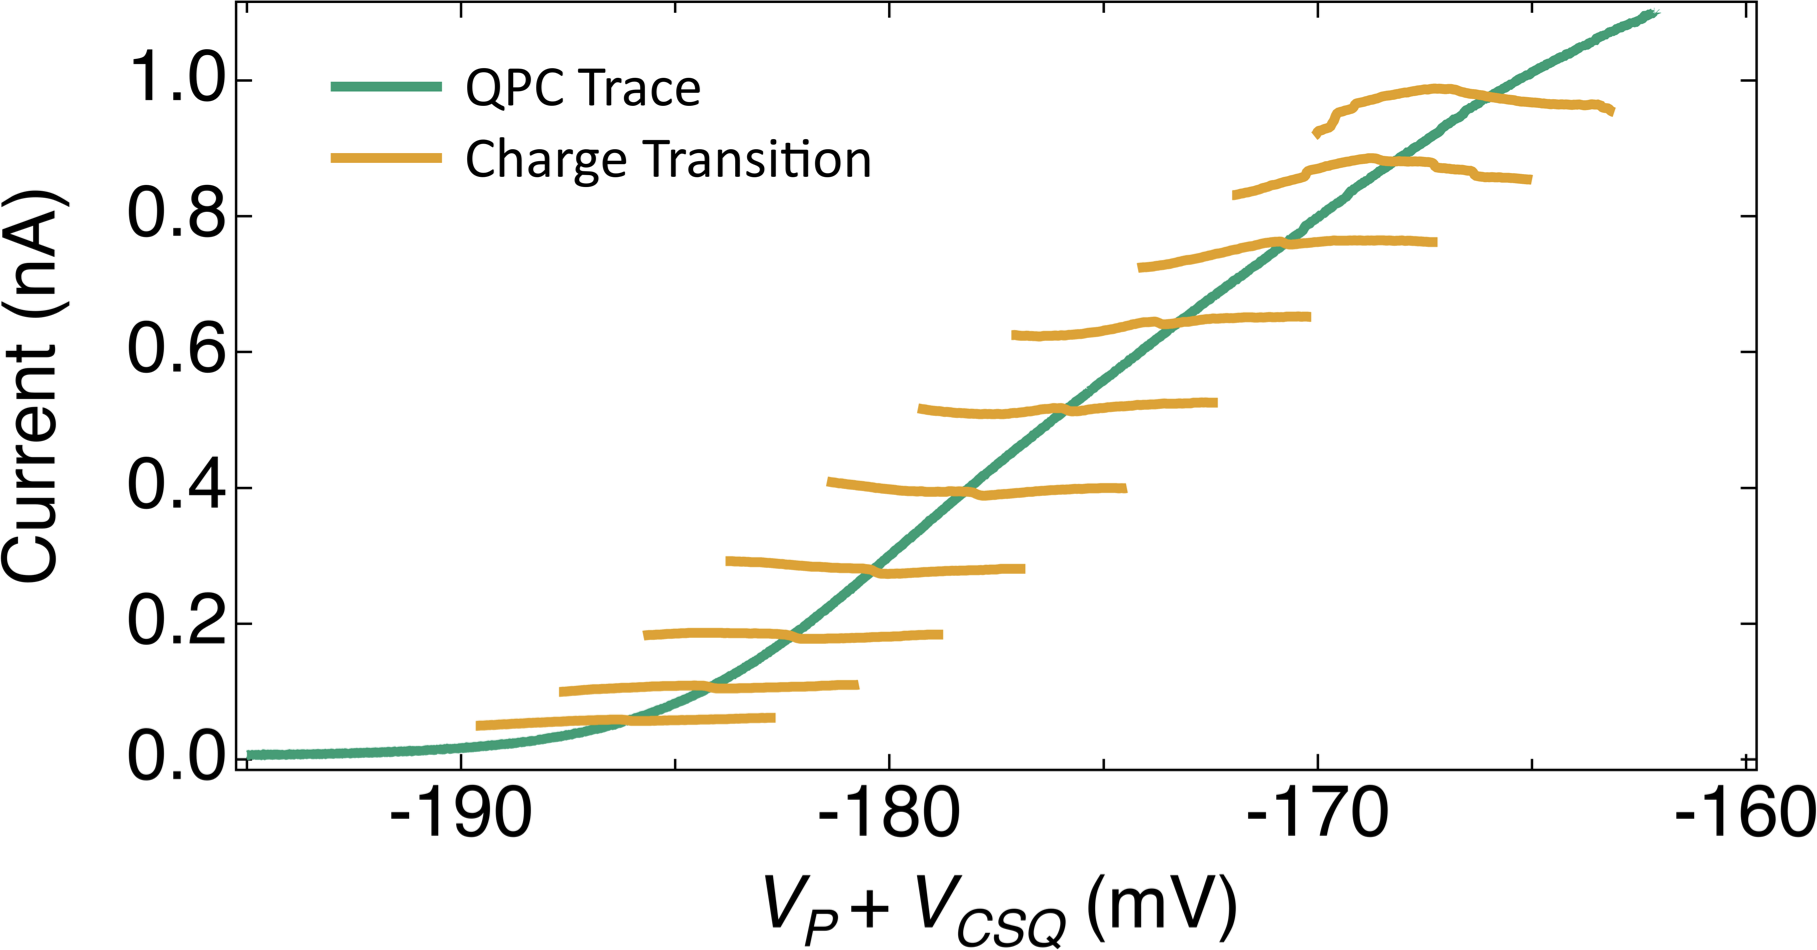
\includegraphics[width=0.8\textwidth]{figures/ch3/crop_FiguresMaster.016.png}
 \caption[Charge transitions measured at various current setpoints through the charge sensor]{\label{fig:ch3/cond_occ_ct_set-points} 
 % For some options that work with pdf\LaTeX, please see this discussion:
 % \url{http://tex.stackexchange.com/questions/11839}. 
 Current through the charge sensor (green) from pinch-off to the start of the first conductance plateau. Corresponding charge transition (yellow) at each of the current setpoints through the charge sensor. Note, the x-axis is not the same between the underlying QPC trace and charge transitions. The charge transitions x-axis has been scaled the same amount for clarity. As the current through the charge sensor is changed, the charge transitions vary dramatically. The left and right slopes curve upwards, downwards, in the same direction, or opposite to each other.}
 \end{center}
\end{figure}
\FloatBarrier

Yet, at each charge sensor current setpoint, the charge transition slopes vary differently on the unoccupied side versus the occupied side. Comparing the slopes on the unoccupied side (left side), at low currents, they point downwards, then point upwards with increasing current, and then point downwards again at the highest current setpoint. It is important to show that the conduction versus occupation agrees with NRG, irrespective of the current setpoint through the charge sensor. Otherwise, it may be possible to `pick' a current setpoint through the charges sensor that shows or does not show agreement with NRG. This would render the method unreliable. 




\subsection{Conductance versus Occupation Varying Charge Sensor Current}



\begin{figure}[!bht]
 \begin{center}
%% includegraphics: comment the following if not using the graphicx package
 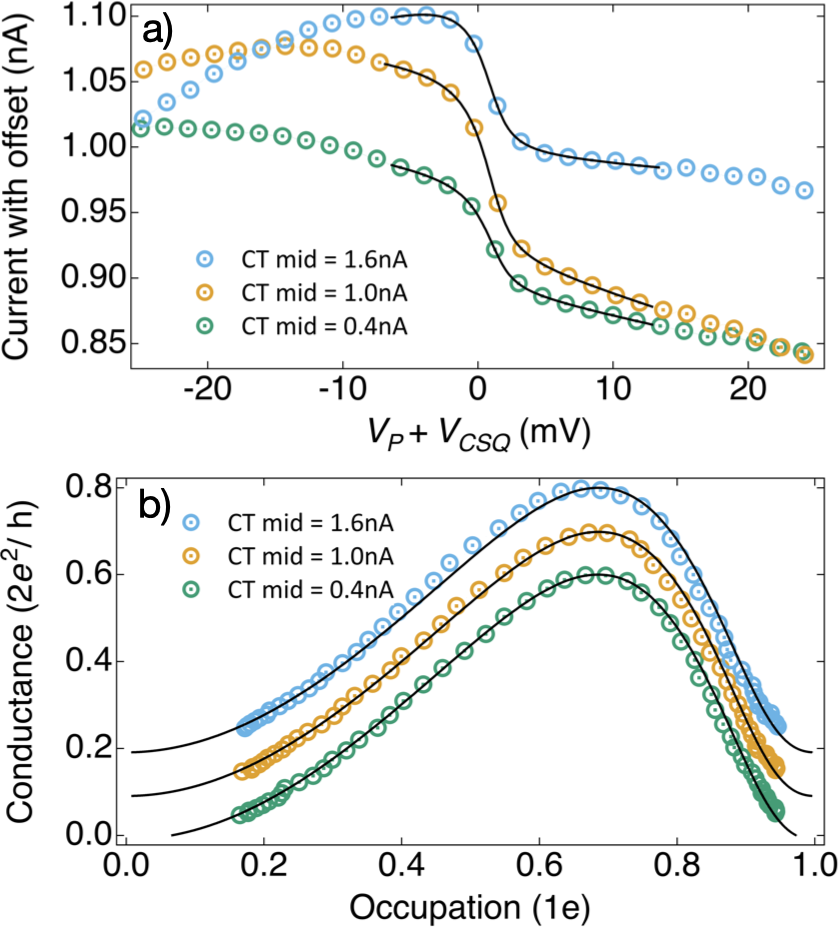
\includegraphics[width=0.8\textwidth]{figures/ch3/crop_FiguresMaster.017.png}
 \caption[Conductance vs. Occupation : Varying the current through the charge sensor]{\label{fig:ch3/cond_occ_QPC_vs_ct} 
 % For some options that work with pdf\LaTeX, please see this discussion:
 % \url{http://tex.stackexchange.com/questions/11839}. 
 (\textbf{a}) Charge transitions are measured with high (blue) and low (green) current through the charge sensor. The transitions are offset in the current for clarity. The x-axis uses the same virtual gate for each charge transition. The slopes on either side of the charge transitions vary with the current through the charge sensor, suggesting the best virtual gate also changes. (\textbf{b}) Conductance versus occupation ($\mathrm{\Gamma/k_BT=21}$) at different current setpoints through the charge sensor. The traces are offset for clarity. Each trace is taken at \qty{20}{mK}. The coupling strength $\mathrm{\Gamma/k_BT}$ was determined from a global fit to conductance at multiple temperatures. The NRG (grey) conductance versus occupation, corresponding to the determined $\mathrm{\Gamma/k_BT}$ is plotted on top of the data. Good agreement is found at each current setpoint.}
 \end{center}
\end{figure}


Fig.~\ref{fig:ch3/cond_occ_QPC_vs_ct}\textbf{a} shows charge transitions taken at \qty{20}{mK}, for three different current setpoints through the charge sensor QPC. Each charge transition has been offset in the current for clarity. Here, it is clear that the shape of the charge transition depends on the current through the charge sensor QPC. The unoccupied (left) side of the high current (blue) charge transition slopes down, whilst the low current (green) charge transition slopes upwards. This suggests that the optimal virtual gate to keep the charge sensor current constant also changes. At each of the current setpoints, conductance was simultaneously measured at a range of temperatures. A global fit to the conductance was used to determine $\mathrm{\Gamma/k_BT}$ and leverarm. Each charge transition was converted into an occupation and the conductance versus occupation is plotted with a comparison to NRG Fig.~\ref{fig:ch3/cond_occ_QPC_vs_ct}\textbf{b}. The conductance versus occupation traces have been offset \qty{0.1}{2e^2/h} for clarity. Excellent agreement between data and NRG is found at each current setpoint. 


% \afterpage{\clearpage}
\section{Varying Coupling Symmetry}

All previous conductance data shown in this thesis was taken with symmetric coupling ($\mathrm{\Gamma_R = \Gamma_L}$). Previous measurements of the Kondo effect have tuned the quantum dot to be symmetrically coupled between the dot and source and drain reservoirs. Although, there have been studies that investigated the Kondo effect with asymmetric coupling ($\mathrm{\Gamma_R \neq \Gamma_L}$)~\cite{kondo_asymmetric}. It was found that the characteristic zero-bias peak in between two conductance peaks shifted to nonzero bias. However, due to the less strong coupling regime explored in this thesis, a zero bias peak is not measured in between two conductance peaks. Although, it is still an interesting experiment to measure the Kondo enhancement as the coupling is varied from symmetric, to asymmetric. This effectively tests how the Kondo enhancement varies when a quantum dot is coupled to two leads (symmetric case) versus a single lead (asymmetric case). In practice, the limit of a single lead regime cannot be reached, as conductance will not be measured through the quantum dot.


% \afterpage{\clearpage}
\subsection{Determining Coupling Symmetry Ratio}


\begin{figure}[!bht]
 \begin{center}
%% includegraphics: comment the following if not using the graphicx package
 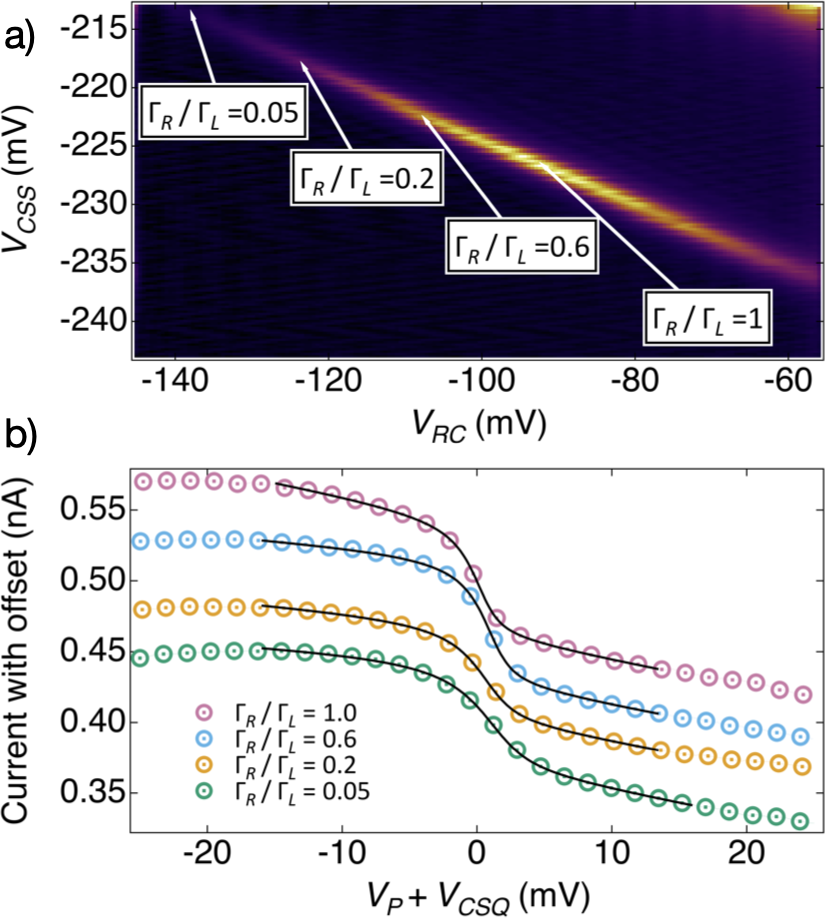
\includegraphics[width=0.8\textwidth]{figures/ch3/crop_FiguresMaster.018.png}
 \caption[Varying coupling symmetry]{\label{fig:ch3/symmetry_picking} 
 % For some options that work with pdf\LaTeX, please see this discussion:
 % \url{http://tex.stackexchange.com/questions/11839}. 
 (\textbf{a}) A 2d scan of conductance through the quantum dot, varying the two coupling gates V\textsubscript{CSS} and V\textsubscript{RC}. In the top left, the dot is more coupled to the right reservoir than the left, $\mathrm{\Gamma_R} = 0.009\cdot\mathrm{\Gamma_L}$. In the middle of the scan (where the conductance is maximum), the coupling is symmetric $\mathrm{\Gamma_R} = \mathrm{\Gamma_L}$ (\textbf{b}) Charge transitions measured with different ratios of coupling between the two leads in the dot. $\mathrm{\Gamma_R/\Gamma_L} = 1.0$ is symmetric coupling (pink), $\mathrm{\Gamma_R/\Gamma_L} = 0.009$ is asymmetric coupling (green). The transitions are offset in the current for clarity. But have been measured with roughly the same current setpoint through the QPC ($\sim\qty{0.4}{nA}$). The x-axis uses the same virtual gate for each charge transition. 
 % The charge transitions become more strongly coupled as asymmetric increases (pink-green)
 }
 \end{center}
\end{figure}


The width of a strongly coupled conductance peak is controlled by $\Gamma$. Where $\Gamma$ is the sum of the individual tunneling rates, $\Gamma=\mathrm{\Gamma_L} + \mathrm{\Gamma_R}$. The amplitude of the conductance depends on the individual tunneling rates Eq.~\ref{eq:cond_amp}. The relation for the overall tunneling rate and conductance amplitude can be re-arranged to express the ratio of tunneling between each lead $\mathrm{\Gamma_L}/\mathrm{\Gamma_R}$.



\begin{equation}\label{eq:cond_ratio}
 \frac{\mathrm{\Gamma_L}}{\mathrm{\Gamma_R}} = 
 \frac
 {\Gamma/2 - \sqrt{\Gamma^2/4 - \Gamma\mathrm{G_0}}}
 {\Gamma/2 + \sqrt{\Gamma^2/4 - \Gamma\mathrm{G_0}}}
\end{equation}


Eq.~\ref{eq:cond_ratio} can be used to show the dot is symmetrically coupled when $\mathrm{\Gamma_L}/\mathrm{\Gamma_R} = 1$, more strongly coupled to the left reservoir when $\mathrm{\Gamma_L}/\mathrm{\Gamma_R} > 1$ and more strongly coupled to the right reservoir when $\mathrm{\Gamma_L}/\mathrm{\Gamma_R} < 1$. To vary the coupling symmetry in a device, a 2d scan measuring the conductance, with a gate that controls a coupling on each axis is used. In Fig.~\ref{fig:ch3/symmetry_picking}\textbf{a}, V\textsubscript{CSS} (y axis) mainly controls $\mathrm{\Gamma_R}$ and V\textsubscript{RC} (x axis) mainly controls $\mathrm{\Gamma_L}$. Four points are picked from symmetric coupling to asymmetric coupling where the dot is more strongly coupled to the right lead. The ratio $\mathrm{\Gamma_L}/\mathrm{\Gamma_R}$ was only calculated after the conductance global fit to NRG, which determined $\Gamma$. 

The charge transitions were simultaneously measured, so that conductance versus occupation could be compared with the corresponding NRG. Charge transitions for each coupling setpoint were measured with $\sim\qty{0.4}{nA}$ through the charge sensor Fig.~\ref{fig:ch3/symmetry_picking}\textbf{b}. Each of the charge transitions did not have charge motion near the transition and were deemed a reliable measure of the occupation. It is interesting that a more asymmetrically coupled transition (green), is more broadened than the symmetrically coupled transition (pink). $\mathrm{\Gamma/T}$ determined from the global fit to conductance varied from 20.5 for symmetric coupling to 26.0 for asymmetric coupling. However, a global fit to the charge transitions finds 19.6 for symmetric coupling and 45.0 for asymmetric coupling Table~\ref{tab:sym_coupling_gf}. 
% \newcolumntype{P}[1]{>{\centering\arraybackslash}p{#1}}

\begin{table}[H] 
\centering
\begin{tabular}{|c|c|c|}
% \begin{tabular}{|c{2.0cm}|c{5.0cm}|c{5.0cm}|}
\hline
 $\mathrm{\Gamma_L}/\mathrm{\Gamma_R}$ & $\mathrm{\Gamma/T}$ Conductance Global Fit & $\mathrm{\Gamma/T}$ Charge Transition Global Fit\\
\hline
0.009 & 26.0 & 45.0\\
0.030 & 24.4 & 30.9\\
0.200 & 22.0 & 21.6 \\
1.000 & 20.5 & 19.6 \\
\hline
\end{tabular}
 \caption[$\mathrm{\Gamma/T}$ determined from a global fit to conductance and charge transitions at different ratios of coupling symmetry.]{\label{tab:sym_coupling_gf} $\mathrm{\Gamma/T}$ determined from a global fit to conductance and separately a global fit to charge transitions at different ratios of coupling symmetry. At symmetric coupling the determined $\mathrm{\Gamma/T}$ from conductance and charge transitions is similar. However, at asymmetric coupling the $\mathrm{\Gamma/T}$ from a global fit to charge transitions is much greater than from a global fit to conductance.}
\end{table}

\afterpage{\clearpage}
\subsection{Conductance versus Occupation Varying Coupling Symmetry}



\begin{figure}[!bht]
 \begin{center}
%% includegraphics: comment the following if not using the graphicx package
 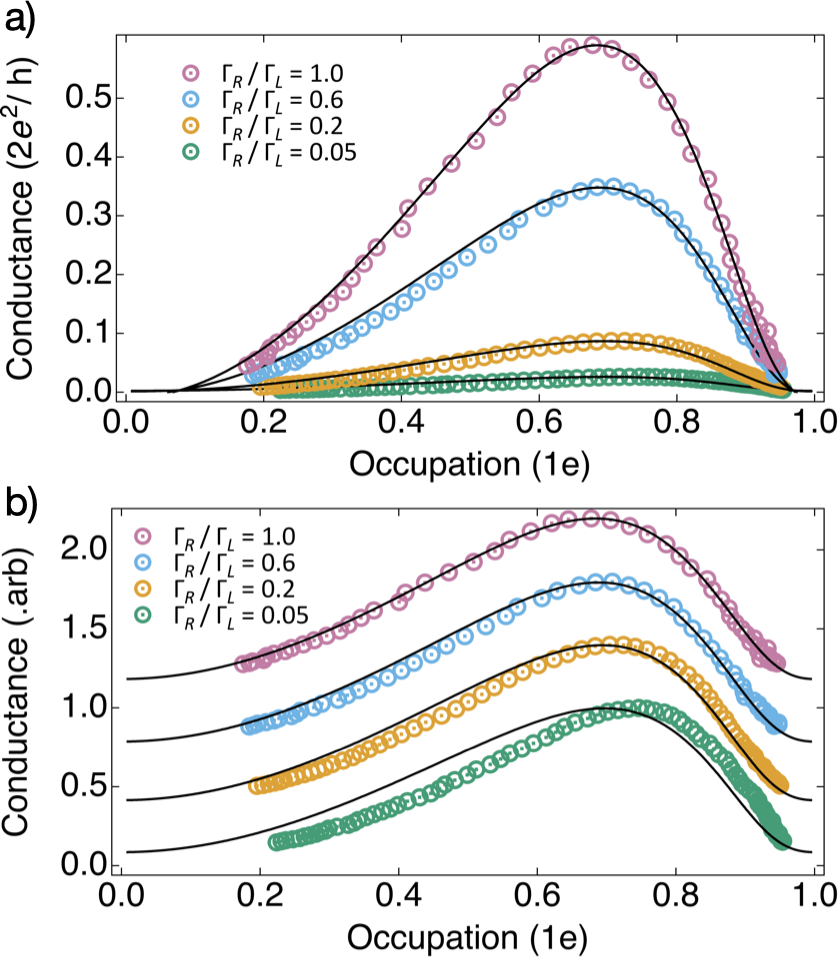
\includegraphics[width=0.8\textwidth]{figures/ch3/crop_FiguresMaster.019.png}
 \caption[Conductance vs. Occupation : Varying the coupling symmetry]{\label{fig:ch3/cond_occ_assymetry} 
 % For some options that work with pdf\LaTeX, please see this discussion:
 % \url{http://tex.stackexchange.com/questions/11839}. 
 (\textbf{a}) Conductance versus occupation ($\mathrm{\Gamma/k_BT=21}$) with different ratios of coupling symmetry between the two leads of the dot. As the asymmetric is increased, the conductance decreases.
 (\textbf{b}) Same data as in (\textbf{a}), except the traces are offset and scaled for clarity. Symmetric coupling agrees well with NRG calculations, however, the asymmetrically coupled data is shifted to the right of the predicted NRG. This suggests that $\mathrm{\Gamma/k_BT}$ extracted from the global fit to conductance is lower than expected.}
 \end{center}
\end{figure}


Fig.~\ref{fig:ch3/cond_occ_assymetry}\textbf{a} shows conductance versus occupation taken at \qty{20}{mK} at the four different ratios of coupling symmetry found in Fig.~\ref{fig:ch3/symmetry_picking}\textbf{a}. There is good agreement with NRG in the symmetric coupling (pink). As the coupling becomes more asymmetric, the conductance maximum decreases Eq.~\ref{eq:cond_amp}, and agreement with NRG is difficult to determine. In Fig.~\ref{fig:ch3/cond_occ_assymetry}\textbf{b} the same data has been scaled and offset for clarity. The corresponding NRG was scaled and offset the same as the data. The disagreement between asymmetric coupling (green) data and NRG is now more clear. When asymmetrically coupled, the conductance maximum of the data is shifted to the right of the NRG. This suggests the $\mathrm{\Gamma/T}$ determined from the global fit to conductance is lower than expected. 

Other studies have used a charge sensor as a noise source to de-phase the Kondo singlet~\cite{kondo_controlled_dephasing}. However, in these studies, the bias across the charge sensor was \qty{1200}{\mu V}, twelve times the bias that is used for the charge sensor in this thesis (\qty{100}{\mu V}) and the suppression of the measured conductance was $\sim6\%$. 
% entanglement of the Kondo singlet with a mesoscopic detector ~\cite{entanglement_measurement}
Another study found that for weak coupling between the charge sensor and quantum dot, the spectral weight of the Kondo resonance is reduced, leading to an observable suppression of the conductance. However, the width of the resonance is not affected, suggesting the absence of dephasing~\cite{peculiar_dephasing_of_kondo}. Furthermore, directly calculating NRG for asymmetric coupling is an active area of research~\cite{kondo_nrg_asymmetric}.




% \clearpage
% \section{Discussion}



